\documentclass[a4paper, 12pt]{report}
\usepackage{geometry}
\usepackage{setspace}
\geometry{
  textheight = 40\baselineskip,
  outer = 20mm,
  inner = 20mm
}
\usepackage[utf8]{inputenc}
\usepackage{fancyvrb}
\usepackage[italian]{babel}
\usepackage[T1]{fontenc}
\usepackage{graphicx}
\usepackage{underscore}
\usepackage{float}
\usepackage{hyperref}
\usepackage{newlfont}
\usepackage{caption}
\usepackage[dvipsnames]{xcolor}
\definecolor{grey}{rgb}{0.5,0.5,0.5}
\hypersetup{
  colorlinks   = true,    % Colours links instead of ugly boxes
  urlcolor     = grey,    % Colour for external hyperlinks
  linkcolor    = grey,    % Colour of internal links
  citecolor    = red      % Colour of citations
}
\newcommand{\source}[1]{\caption*{Fonte: {#1}}}
\textwidth=450pt\oddsidemargin=0pt
\begin{document}
\documentclass[12pt,a4paper]{report}
\usepackage[italian]{babel}
\usepackage{newlfont}
\textwidth=450pt\oddsidemargin=0pt
\begin{document}
\begin{titlepage}
\begin{center}
{{\Large{\textsc{Alma Mater Studiorum $\cdot$ Universit\`a di
Bologna}}}} \rule[0.1cm]{15.8cm}{0.1mm}
\rule[0.5cm]{15.8cm}{0.6mm}
{\small{\bf SCUOLA DI SCIENZE\\
Corso di Laurea in Nome corso di Laurea }}
\end{center}
\vspace{15mm}
\begin{center}
{\LARGE{\bf TITOLO}}\\
\vspace{3mm}
{\LARGE{\bf DELLA}}\\
\vspace{3mm}
{\LARGE{\bf TESI}}\\
\end{center}
\vspace{40mm}
\par
\noindent
\begin{minipage}[t]{0.47\textwidth}
{\large{\bf Relatore:\\
Chiar.mo Prof.\\
NOME RELATORE}}
\end{minipage}
\hfill
\begin{minipage}[t]{0.47\textwidth}\raggedleft
{\large{\bf Presentata da:\\
NOME LAUREANDO}}
\end{minipage}
\vspace{20mm}
\begin{center}
{\large{\bf Sessione\\%inserire il numero della sessione in cui ci si laurea
Anno Accademico }}%inserire l'anno accademico a cui si � iscritti
\end{center}
\end{titlepage}
\end{document}

\graphicspath{ {./} }
\setstretch{1.2}
\setlength{\parindent}{0em}
\setcounter{secnumdepth}{0}
\makeatletter
\renewcommand\section{\@startsection{section}{1}{\z@}%
                                   {-3.5ex \@plus -1ex \@minus -.2ex}%
                                   {2.3ex \@plus.2ex}%
                                   {\normalfont\large\bfseries\center}}
  \hyphenation{ON-DELETE GraphQL AbstractMongooseDAO Type-Script}
  \section{Introduzione}
    \paragraph*{}
      La storia dello standard \emph{JSON}, dei database documentali e la necessità di sviluppare tecnologie per interagirci devono in buona parte la loro diffusione al mondo dello sviluppo Web.
      Sin dagli anni novanta infatti, nel mercato dei web browser, era presente il bisogno di creare pagine più dinamiche e interagibili; a questo scopo fu sviluppato \emph{JavaScript}, linguaggio di scripting per browser capace di interagire con la struttura delle pagine ed inviare richieste ad altre macchine.
    \paragraph*{}
      Con lo sviluppo di applicazioni web sempre più visualmente ricche, l'industria si è trovata davanti al problema di dover trasferire fra front-end e server informazioni su oggetti dalla crescente complessità.
      È per questo che, in modo indipendente, nei primi anni duemila si diffusero tecniche di trasferimento di oggetti tramite HTTP utilizzando la notazione per gli oggetti \emph{literal} del linguaggio JavaScript.
      Queste tecniche, nate in modo spontaneo e scoordinato, vennero poi condensate e definite nello standard JSON per la rappresentazione di oggetti.
      Il JSON oggi è diffuso in qualsiasi applicazione Web, vista la facilità di interpretazione del suo formato, supportato da molti linguaggi, fra cui ovviamente il JavaScript.
      \paragraph*{}
      Un altro campo nel quale questo formato ha ottenuto un grande successo è quello dei Database \emph{NoSQL}, in particolare quelli documentali: salvare informazioni provenienti dal web già in formato JSON è diventata una pratica diffusa, anche perché spesso i contenuti di applicazioni web non sono facilmente descrivibili in modo strutturato, prerequisito per l'utilizzo di database \emph{relazionali} SQL, l'altro paradigma di archiviazione più diffuso.
    \paragraph*{}
      I database relazionali documentali incorrono però in due importanti limiti:
      \begin{itemize}
        \item Mentre le relazioni "in verticale" (gerarchie) sono rappresentabili, i documenti non supportano quelle fra documenti diversi. Non è infatti presente di norma un meccanismo simile a quello delle chiavi per SQL.
        \item Non è mai stato definito o adottato un linguaggio di interrogazione e modifica unificato per i database documentali.
      \end{itemize}
    \paragraph*{}
      Per questo, Facebook attorno al 2012 decise di iniziare a progettare e sviluppare \emph{GraphQL}, un linguaggio per API ideato per descrivere operazione di lettura e scrittura di dati.
    \paragraph*{}
      La spinta verso la definizione di questo linguaggio è stata data da alcune necessità derivate anche dalle limitazioni dei database documentali sopra indicate:
      \begin{itemize}
        \item Facebook faceva largo uso del formato JSON per il salvataggio di informazioni: cambiare l'infrastruttura sottostante sarebbe risultato troppo costoso;
        \item i dati gestiti da Facebook come post, utenti, commenti e reazioni risultano meglio rappresentabili da database non relazionali;
        \item allo stesso tempo, il valore di questi dati risiede nelle relazioni fra di essi (ad esempio, quali utenti sono amici di altri).
      \end{itemize}
    \paragraph*{}
      Caratteristica fondamentale di GraphQL è la possibilità di definire uno schema che permette di modellare il formato delle \emph{query} esposte e quello delle \emph{entità} sulle quali operare con esse, di modo che il client possa effettuare richieste personalizzate ad un singolo endpoint ricevendo in risposta dati già tipizzati.
      Le entità sono definite da campi tipizzati e relazioni con altre entità, la struttura del dominio delle interrogazioni gestibili dal server è strutturata come un grafo.
    \paragraph*{}
      Il linguaggio, pubblicato nel 2015, è dal Novembre del 2018 uno standard\footnote{http://spec.graphql.org/} e la sua gestione è stata trasferita da Facebook alla \emph{GraphQL Foundation}, sotto l'ala della \emph{Linux Foundation}.
      Grazie alla sua maturazione degli ultimi anni, allo sviluppo di servizi costruiti per implementarlo ed alla sua adozione da parte di numerose aziende\footnote{https://landscape.graphql.org/card-mode?category=graph-ql-adopter\&grouping=category}, GraphQL si presenta oggi come uno standard capace di competere con l'architettura di tipo REST per il dialogo fra client e server.
    \paragraph*{}
      Le possibilità offerte dallo standard però non si limitano alla comunicazione fra client e server: essendo i campi delle entità tipizzati, ed avendo lo standard un concetto di introspection, è possibile usare 
      schemi GraphQL anche per definire lo strato del model.
      Questa possibilità rende quindi l'impiego di questo standard potenzialmente adatto per lo sviluppo Model Driven, permettendo di generare in modo automatizzato il codice applicativo che si occuperà di interfacciarsi con le strutture definite nello schema GraphQL.
    \paragraph*{}
      \textbf{Twinlogix S.r.l}, azienda di Santarcangelo di Romagna, recentemente espansa anche a Cesena, ha seguito con interesse la maturazione dello standard GraphQL e in questo momento sta ponendo fra gli obiettivi interni il passaggio completo da API Rest a GraphQL.
    \paragraph*{}
      Fra le sue occupazioni ci sono lo sviluppo di sistemi software in ambiente Web e Mobile e nel 2013 ha fatto nascere anche un'altra azienda imparentata: \emph{Cassanova}.
      Questa offre come prodotto di punta \emph{CassaInCloud}, sistema software per attività commerciali in grado di fornire diversi servizi, dalla gestione dei turni all'e-commerce.
    \paragraph*{}
      Fra gli altri obiettivi interni dell'azienda c'è anche quello di aggiornare le tecnologie di generazione di codice sviluppate in passato, realizzate con tecnologie proprietarie dalla documentazione, supporto e diffusione limitati.
      Prestandosi facilmente alla descrizione di modelli da generare automaticamente, GraphQL risulta anche un ottimo strumento per la scrittura del nuovo generatore di codice.
    \paragraph*{}
      Twinlogix ha quindi deciso di sfruttare questa potenzialità per realizzare un generatore di codice che, basandosi su uno schema GraphQL, costruisca definizioni di modelli per database.
      Per poter interagire con questi modelli il generatore deve anche generare i DAO necessari.
      A tal scopo, l'azienda sta lavorando anche alla scrittura di un DAO generico e metodi per interagirci indipendenti dal tipo dell'oggetto richiesto e dal database sottostante.
      È stato già scritto un primo prototipo di questo DAO e di una versione del generatore indirizzata a database MongoDB.
    \paragraph*{}
      Obiettivi dell'attività discussa in questo documento sono stati quindi:
      \begin{itemize}
        \item studiare le tecnologie necessarie per lo svolgimento dell'attività;
        \item analizzare l'architettura del DAO e i prototipi sviluppati dall'azienda;
        \item progettare e implementare una prima versione del DAO generico e del generatore che, sfruttando librerie ORM, potesse interfacciarsi con database SQL.
      \end{itemize}
    \renewcommand\section{\@startsection{section}{1}{\z@}%
    {-3.5ex \@plus -1ex \@minus -.2ex}%
    {2.3ex \@plus.2ex}%
    {\normalfont\large\bfseries}}
  \newpage
  \tableofcontents
  \newpage
  \listoffigures
  \addcontentsline{toc}{chapter}{Elenco delle figure}
  \chapter{Contesto tecnologico}
    \section{Model Driven Programming}
      Lo sviluppo "Model Driven" è un approccio all'ingegneria del software orientato alla definizione di modelli piuttosto che di software.
      \paragraph*{}
      La complessità di un progetto può essere catalogata in due macro gruppi:
      \begin{itemize}
        \item \emph{essenziale}, ovvero derivata dal problema che si cerca di risolvere, indipendente dalle tecnologie impiegate;
        \item \emph{accidentale}, dovuta agli strumenti impiegati per affrontare il problema.
      \end{itemize}
      \paragraph*{}
      Uno degli obiettivi di una buona progettazione è quello quindi di ridurre il più possibile la complessità accidentale.
      La complessità di molti sistemi software moderni è talmente elevata da renderne difficile sia la comprensione (basandosi solo sul codice scritto), sia la realizzazione: parlare di modelli permette di rendere comprensibile l'architettura di un progetto e di potersi concentrare sugli obiettivi, dimenticandosi delle complicazioni e limitazioni che verrebbero incontrate in fase di sviluppo.
      \paragraph*{}
      La programmazione in sé è un'attività con un'alta potenzialità di errori accidentali: una sola riga di codice sbagliata è infatti sufficiente per causare costosi danni \footnote{http://users.csc.calpoly.edu/~jdalbey/SWE/Papers/att_collapse}.
      \paragraph*{}
      Spesso, in fase di implementazione di sistemi complessi, ci si trova poi davanti a blocchi di codice strutturati in modo estremamente ripetitivo e complesso: questa è una situazione nella quale errori accidentali sono quasi assicurati.
      In questo tipo di sezioni la modellazione può incontrare facilmente la generazione di codice: questi blocchi di codice possono essere descritti in modo astratto ed indipendente da linguaggi di programmazione e librerie.
      \paragraph*{}
      Utilizzare questo approccio dove utile porta a notevoli benefici:
      \begin{itemize}
        \item il tempo e le forze degli ingegneri sono utilizzati in modo migliore: tutta la complessità dell'implementazione è spostata sulla scrittura dei generatori di codice, piuttosto che di sezioni ripetitive;
        \item un progetto strutturato con modelli diventa più comprensibile anche per il cliente;
        \item in caso siano necessarie modifiche, basterà effettuarle al modello. I cambiamenti sono poi generati rapidamente e senza rischio di errori accidentali.
      \end{itemize}
    \section{ORM}
      L'\emph{Object Relational Mapping} è una tecnica di programmazione creata per favorire l'interazione fra un'applicazione scritta con un approccio ad oggetti ed una base di dati di tipo relazionale, o comunque modellante tabelle tramite campi scalari semplici.
      Una libreria ORM rende quindi possibile mappare le tabelle in oggetti e viceversa, permettendo di poter operare con questi dentro l'applicazione anche quando si deve comunicare con un DB.
    \paragraph*{}
      Esempio di confronto fra l'utilizzo di un driver DB e quello di una libreria ORM (fonte snippets: \href{https://en.wikipedia.org/wiki/Object%E2%80%93relational_mapping}{en.wikipedia.org}):
      \begin{Verbatim}[samepage=true]
        // Versione utilizzante il driver del DB
        {
          var sql = "SELECT * FROM persons WHERE id = 10";
          var result = context.Persons.FromSqlRaw(sql).ToList();
          var name = result[0]["first_name"];
        }
      \end{Verbatim}
      \begin{Verbatim}[samepage=true]
        // Versione utilizzante una libreria ORM
        {
          var person = Person.Get(Person.Properties.Id == 10);
          var firstName = person.GetFirstName();
        }
      \end{Verbatim}
      Gli immediati vantaggi di questo approccio sono il ridotto numero di righe di codice scritte e la conseguente pulizia del codice, nonché la semplicità nell'interazione con il DB e la minor probabilità di errore, non dovendo scrivere esplicitamente interrogazioni in linguaggio SQL.
      D'altro canto, utilizzare una libreria ORM ha anche svantaggi:
      \begin{itemize}
        \item è una libreria complessa se la si vuole sfruttare a fondo;
        \item toglie del controllo al programmatore, vista la grande astrazione che introduce;
        \item produce query sub-ottimali rispetto ad una persona esperta di SQL.
      \end{itemize}
      Questi svantaggi non sono però stati ritenuti abbastanza influenti da decidere di optare per una soluzione di più basso livello.
    \section{GraphQL}
      Ideato da Facebook nel 2012, il linguaggio GraphQL è stato successivamente pubblicato in maniera open source e, dal 2018, è gestito come standard dalla GraphQL Foundation.
      Nasce con il duplice scopo di modellare entità collegate fra di loro da relazioni e di fornire una soluzione a noti problemi dell'approccio RESTful, architettura per la comunicazione client server prevalente nello sviluppo in ambito web.
      \subsection{Tipi di base}
      Il linguaggio di GraphQL permette di definire uno schema costituito dai tipi:
        \paragraph*{Oggetto} 
          Nodi che rappresentano la struttura delle entità gestite dall'applicativo.
        \paragraph*{}
          Esempio di tipo oggetto: è definito un oggetto nominato "Address" con tre proprietà tipizzate.
          \begin{Verbatim}[samepage=true]
            type Address {
              street: String
              city: String
              country(continent: Continent): Country!
            }
          \end{Verbatim}
          Il nodo contiene due valori scalari ("street" e "city"), mentre la proprietà "country" è di tipo oggetto; questo indica che esiste un collegamento fra il nodo Address e quello Country. Si nota anche come le proprietà possano ricevere dei parametri in input.
          Il carattere '\emph{!}' indica che il campo dell'entità è non nullo.
        \paragraph*{Query e mutazioni} 
          Richieste che il client può effettuare al server. Rappresentano i punti d'ingresso nel grafo (dopo il nodo root, implicitamente incluso). Le \emph{query} rappresentano operazioni di lettura, mentre le \emph{mutations} quelle di modifica.
        \paragraph*{}
          Definizione delle keyword \emph{query} e \emph{mutation}:
          \begin{Verbatim}[samepage=true]
            schema {
              query: Query
              mutation: Mutation
            }
          \end{Verbatim}
        \paragraph*{}
          Esempio di definizione delle query esposte:
          \begin{Verbatim}[samepage=true]
            type Query {
              address(continent: Continent): Character
              user(id: ID!): User
            }
          \end{Verbatim}
      \subsection{Direttive}
        Per personalizzare ulteriormente l'espressività dello schema, lo standard GraphQL supporta anche l'uso di \emph{direttive}, parole chiave definite nello schema e precedute dal carattere '\emph{@}'. Le direttive possono avere anche degli attributi.
      \paragraph*{}
        Esempi di definizioni e utilizzo di direttive in uno schema:
        \begin{Verbatim}[samepage=true]
          directive @id(auto: Boolean) on FIELD_DEFINITION
          directive @ref(from: String!, to: String) on FIELD_DEFINITION
          directive @entity on INTERFACE | OBJECT | FIELD_DEFINITION

          type MyType @entity {
            id: ID! @id,
            field: String @ref(from: "OtherType") 
          }
        \end{Verbatim}
        In questo esempio vengono definite tre direttive, di cui le prime due applicabili solamente su campi, mentre l'ultima anche su tipi oggetti e interfacce.
        È da notare anche che tutti gli attributi di queste direttive sono opzionali, tranne quello \emph{refFrom} della direttiva \emph{foreignRef}, segnalato con un punto esclamativo dopo il tipo.
      \subsection{Comunicazione con il server}
        Per contattare un server GraphQL, un client può fornire come parametri di richiesta un'operazione di query o mutazione fra quelle definite nello schema, specificandone la forma dell'output.
      \paragraph*{}
        Le immagini successive mostrano un esempio di comunicazione con un server GraphQL in contrasto ad uno implementante l'API REST.
        \begin{figure}[H]
          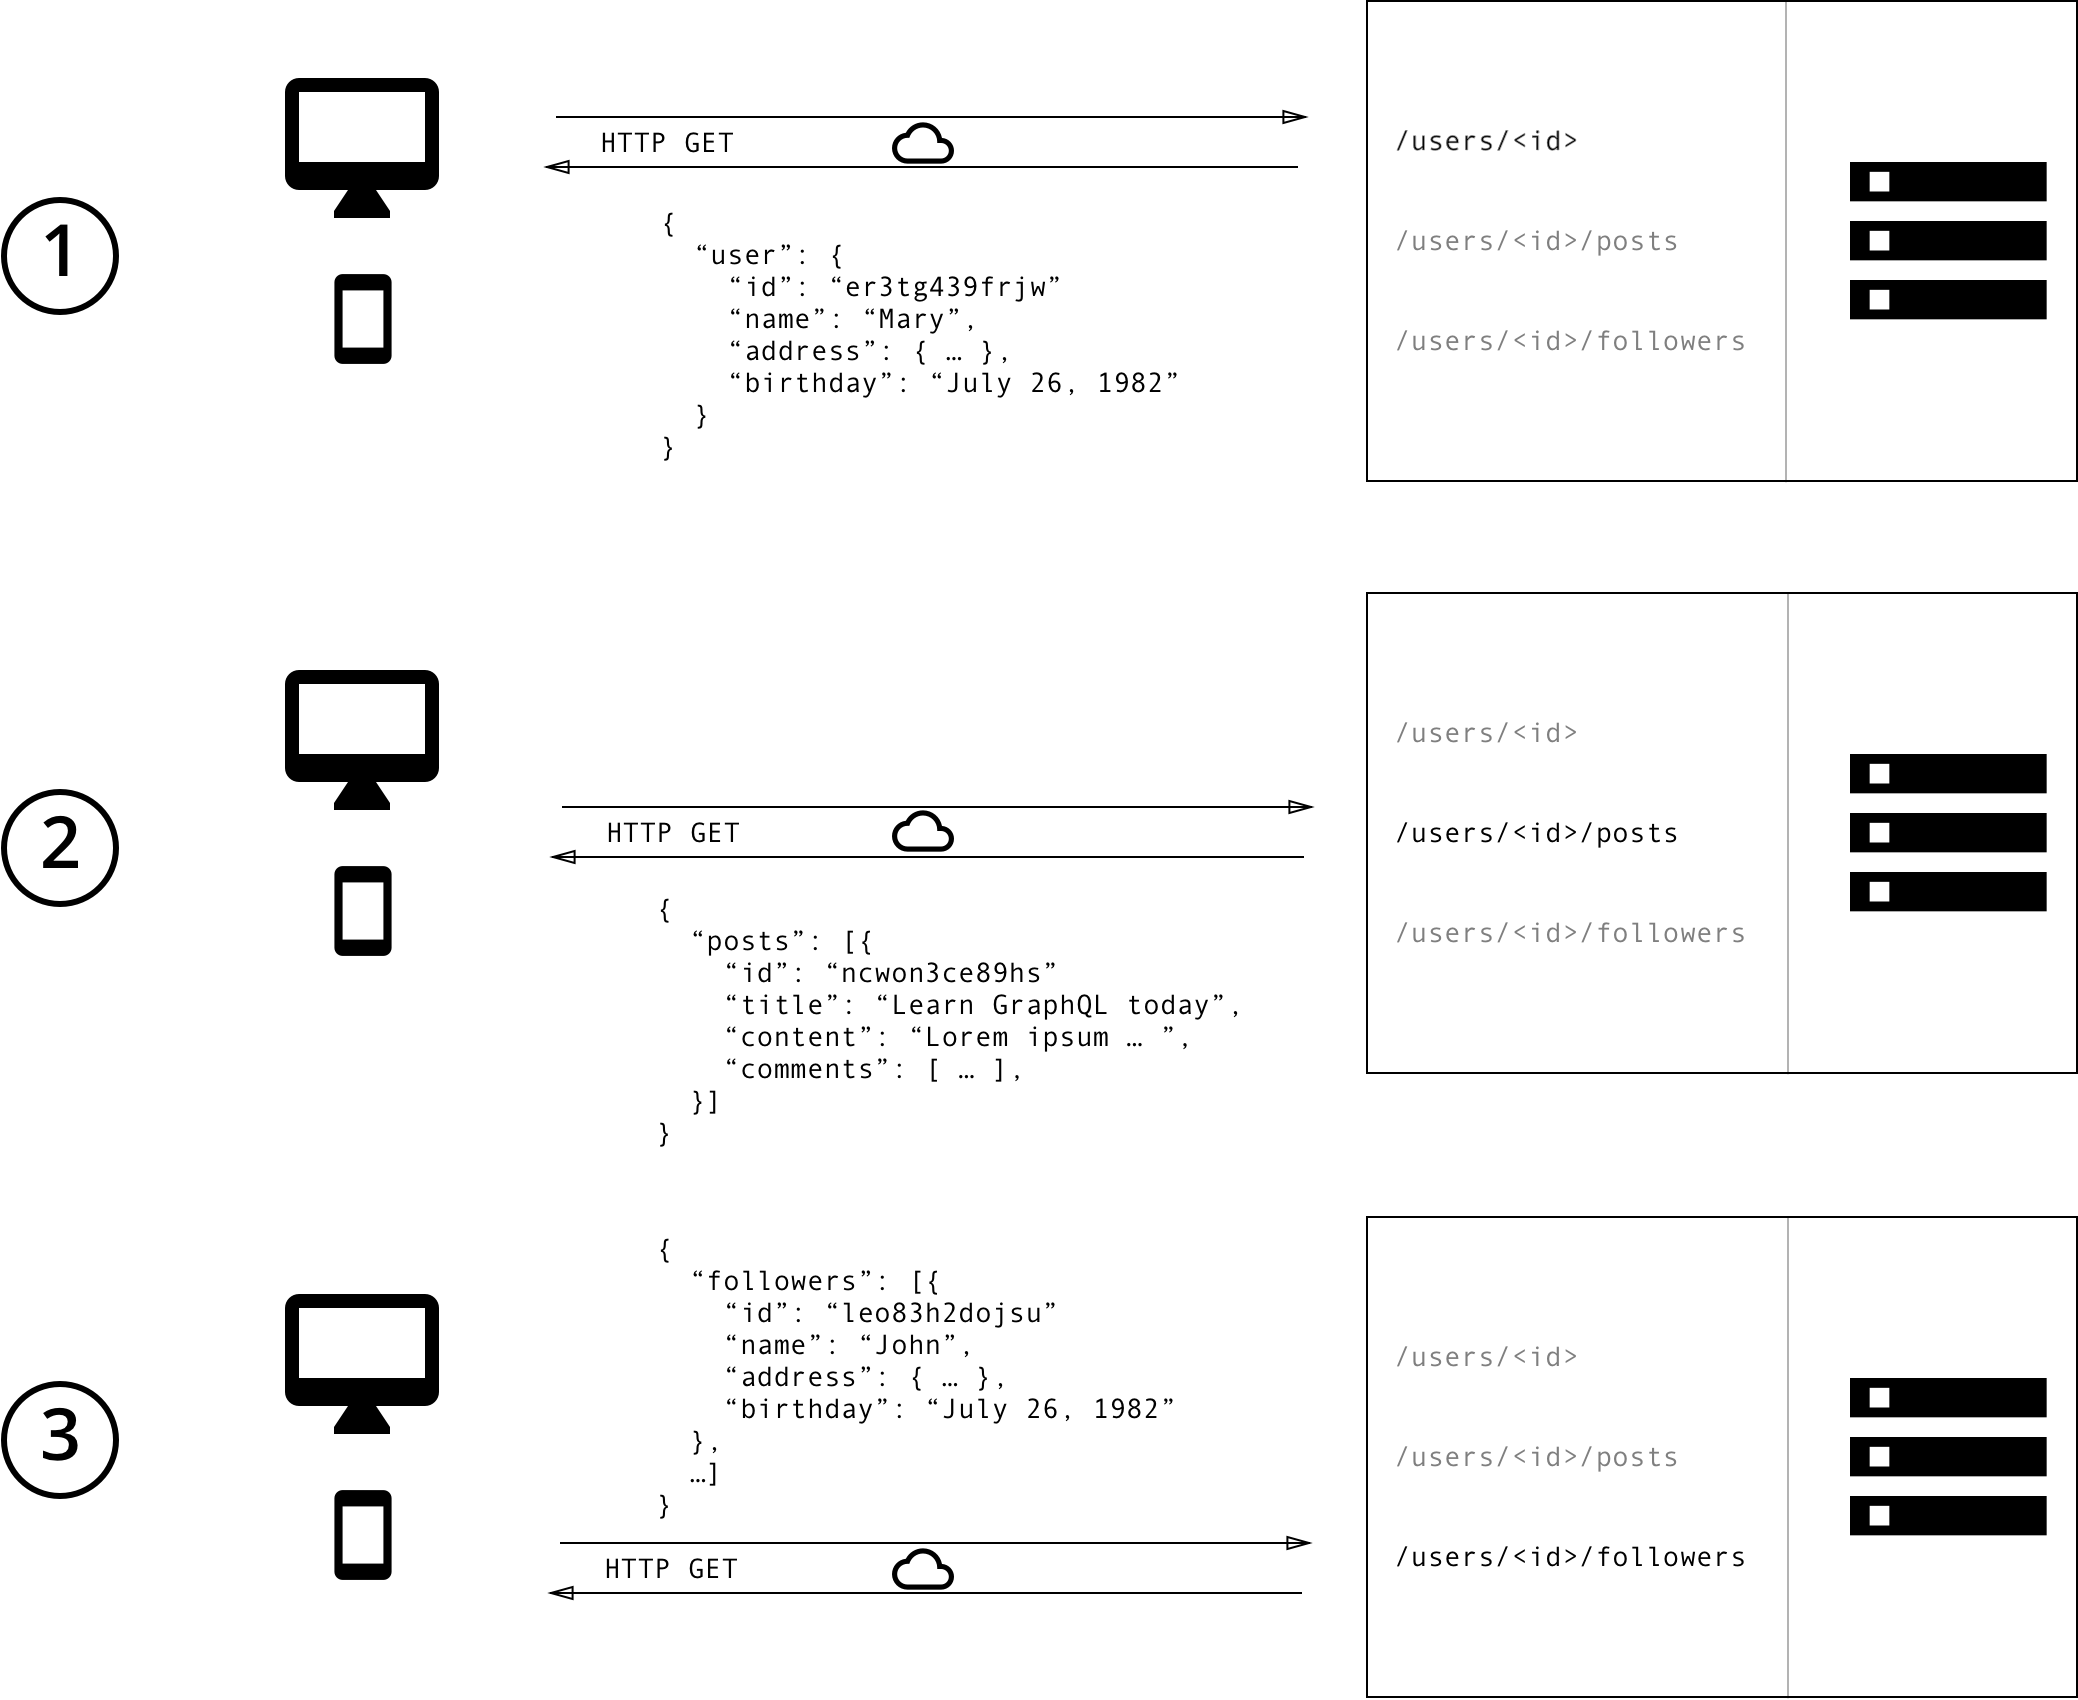
\includegraphics[width=\textwidth]{rest-communication.png}
          \caption{Esempio di comunicazione con server REST.}
          \source{\href{https://www.howtoGraphQL.com/basics/1-GraphQL-is-the-better-rest/}{www.howtographql.com}}
        \end{figure}
        \begin{figure}[H]
          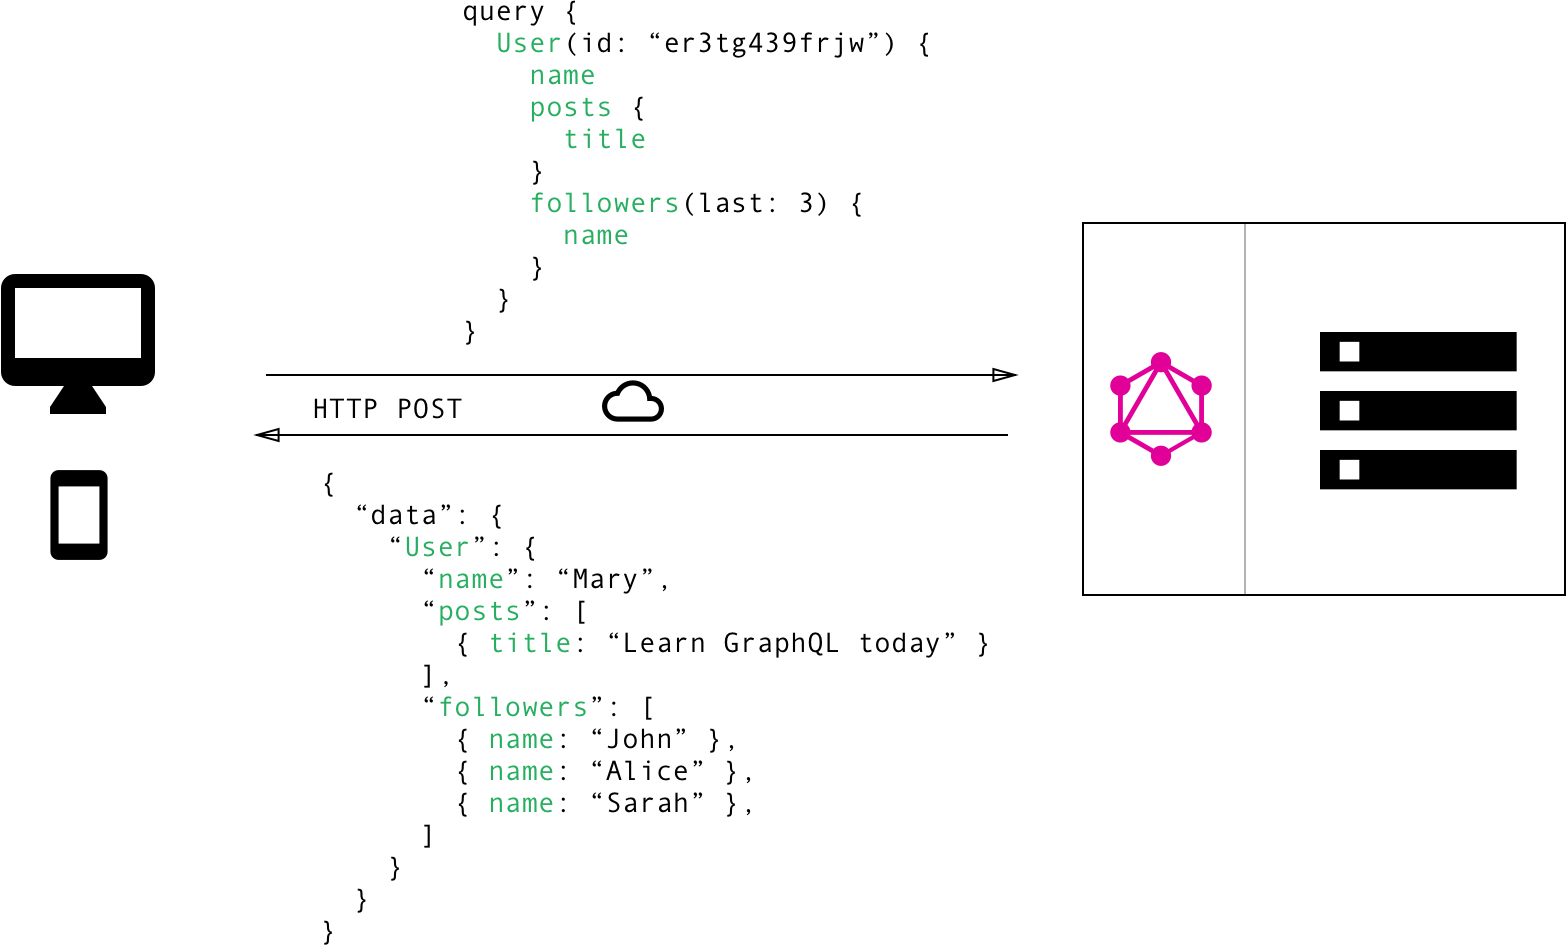
\includegraphics[width=\textwidth]{graphql-communication.png}
          \caption{Esempio di comunicazione con server GraphQL.}
          \source{\href{https://www.howtoGraphQL.com/basics/1-GraphQL-is-the-better-rest/}{www.howtographql.com}}
        \end{figure}
        \paragraph*{}Si nota quindi che l'utilizzo di GraphQL permette di risolvere alcuni problemi dell'approccio REST:
        \paragraph*{Overfetching e underfetching} 
          Ovvero il fatto che, essendo il formato delle risposte del server fisso, il client spesso riceve più (o meno) informazioni di quelle necessarie.
          Nel caso in cui ne riceva meno, la cosa comporta anche la necessità di effettuare altre richieste al server per ricevere i dati necessari.
          Come si può notare dalle immagini di esempio, in una richiesta GraphQL è invece il client a specificare esattamente il formato della risposta.
        \paragraph*{Multipli endpoint}
          Lo schema GraphQL indica un solo punto d'ingresso, il nodo root; da quello si può accedere alle varie query e mutazioni.
          Il fatto che ci sia un solo punto d'ingresso significa che per il client basterà contattare un unico endpoint per ricevere tutte le informazioni di cui ha bisogno.
          Questo è evidenziato nell'immagine di esempio di comunicazione con server REST: il client ha dovuto contattare tre endpoint differenti.
        \paragraph*{Modifiche all'API}
          Il fatto che in un'architettura REST sia il server a dover definire il formato dei risultati di una chiamata comporta che l'API di back-end debba essere modificata spesso per riflettere i cambiamenti nell'interfaccia front-end, se non si vuole
          incorrere in fenomeni di over o underfetching.
          Lo standard GraphQL permette quindi una più rapida produzione di applicazioni e un'API back-end più stabile.
        \paragraph*{Interpretazione dell'output}
          Essendo i campi dei nodi GraphQL tipizzati, i tipi della risposta di un server GraphQL sono inequivocabili: questo facilita la comprensione dell'output di una richiesta.
          Lo standard GraphQL supporta anche il concetto di \emph{introspection}: questo permette, anche senza avere accesso allo schema, di scoprire le query e i formati dei dati.
          Una soluzione REST prevede invece la scrittura e il mantenimento di una documentazione a riguardo.
        \paragraph*{}
          Oltre a fornire uno standard robusto per la comunicazione client server, GraphQL può essere usato come linguaggio per definire modelli: sono infatti già disponibili servizi di generazione di codice basata su schemi GraphQL.
          Quello utilizzato in questo caso è \emph{GraphQL Code Generator}\footnote{https://graphql-code-generator.com/}.
    \section{GraphQL code generator}
      GraphQL code generator è un tool CLI open source in grado di analizzare uno schema GraphQL e, tramite plugins, generare codice su diversi file.
      Il modo in cui i plugin di questo strumento operano segue il pattern di programmazione \emph{visitor}.
      \paragraph*{}
        Il pattern visitor è una soluzione al problema che si verifica quando bisogna effettuare operazioni su una struttura di oggetti senza però aggiungere funzionalità agli stessi:
        ogni oggetto della struttura implementa un'interfaccia definente un metodo \emph{accept} che riceve come parametro un'implementazione dell'interfaccia Visitor.
        Questa specifica invece un metodo \emph{visit} per ogni tipologia di oggetto (ad esempio, ogni classe) sul quale svolgere operazioni.
      \paragraph*{}
        Nell'applicazione principale poi, per ogni oggetto, viene chiamato il metodo accept passando ogni implementazione di Visitor, cosicché per aggiungere operazioni/trasformazioni delle classi è possibile semplicemente implementare un nuovo Visitor.
      \begin{figure}[H]
          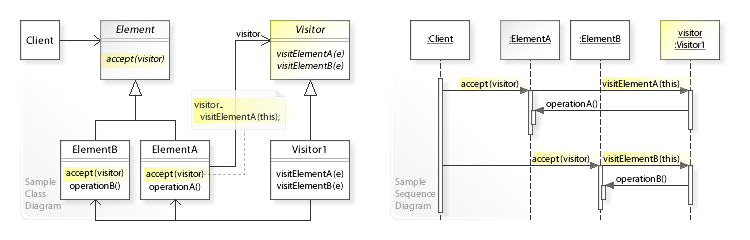
\includegraphics[width=\textwidth]{visitor-example.jpg}
          \caption{Esempio di struttura e funzionamento del pattern Visitor.}
          \source{\href{https://en.wikipedia.org/wiki/Visitor_pattern}{en.wikipedia.org}}
      \end{figure}
      \paragraph*{}È questo il meccanismo alla base di GraphQL code generator: al suo interno, ogni plugin può accedere allo schema del grafo e chiamare il metodo \emph{visit}, passando come parametro un oggetto che funga da visitor.
        Sono disponibili dei plugin predefiniti fra cui quello, usato durante questo progetto, per generare tipi in linguaggio TypeScript basati sulle entità dello schema.
    \section{TypeScript}
      TypeScript è un linguaggio open source ideato per arricchire il linguaggio JavaScript aggiungendo i tipi statici.
      L'uso dei tipi permette la validazione del codice e, di conseguenza, uno sviluppo più fluido.
      \paragraph*{}
      Oltre a definire tipi di base come \emph{number} o \emph{string}, TypeScript supporta anche tipi composti. Ad esempio:
      \begin{Verbatim}[samepage=true]
        type NetworkFromCachedState = {
          state: "from_cache";
          id: string;
          response: NetworkSuccessState["response"];
        };
      \end{Verbatim}
      rappresenta un tipo con tre attributi:
      \begin{itemize}
        \item state: è di tipo "from_cache", ovvero un tipo che accetta solo quel valore. Tipi definiti in questo modo sono detti \emph{literal types}
        \item id: campo di tipo \emph{string}
        \item response: campo di tipo \emph{typeof NetworkSuccessState["response"]}. Il suo tipo corrisponde a quello di un oggetto definito in un altro tipo.
      \end{itemize}
      È possibile creare tipi avanzati, ma la questione non verrà discussa in questo testo.
      \paragraph*{}
      I tipi, a differenza delle classi, non hanno un operatore nativo (come \emph{typeof}) per distinguerli.
      Per controllare il tipo di una variabile è necessario definire \emph{type guards} personalizzate.
      \begin{Verbatim}[samepage=true]
        type stringWrapper = {
          value : string;
        }
        function isString(x: any): x is stringWrapper {
          return typeof x["value"] === "string";
        }
        function printIfString(x : any) {
          if(isString(x)) {
            console.log(x.value);
          }
        }
      \end{Verbatim}
      In questo caso, senza la type guard, cercare di usare la proprietà "x.value" genererebbe un errore di validazione del codice, essendo x di tipo any.
    \section{Sequelize}
      In accordo con l'azienda, la versione SQL è stata scritta sfruttando la libreria ORM per ambiente Node \emph{Sequelize} per l'interazione con la base di dati.
      Sequelize supporta i seguenti RDBMS:
      \begin{itemize}
        \item Postgres
        \item MySQL
        \item MariaDB
        \item SQLite
        \item Microsoft SQL Server
      \end{itemize}
      Descrivere nello specifico il funzionamento della libreria non rientra negli obiettivi di questo documento (alcune funzionalità verranno esposte in seguito) ma, per la comprensione del testo, si introducono di seguito i concetti di \emph{associazione}  e \emph{Model} di Sequelize.
      \paragraph*{Model} 
      I Model sono le entità sulle quali la libreria opera. Sono oggetti che astraggono le tabelle salvate sul database.
      Al loro interno posseggono informazioni sui campi (nome, valore, tipo\dots), sulla tabella (nome della tabella, nome del model, associazioni\dots) etc\dots
      \paragraph*{}
      Mentre una classe statica relativa ad una tabella rappresenta tutta la tabella ed espone metodi per effettuare modifiche e letture in blocco su di essa, un \emph{istanza} di Model rappresenta una riga di una tabella.
      I metodi di modifica riguarderanno solo il record associato a quella istanza.
      \paragraph*{Associazioni}
      Le associazioni sono oggetti usati per gestire le associazioni \emph{uno a uno}, \emph{uno a molti} e \emph{molti a molti} fra tabelle.
      Esistono quattro tipi di associazioni Sequelize:
      \begin{itemize}
        \item HasOne
        \item BelongsTo
        \item HasMany
        \item BelongsToMany
      \end{itemize}
      \paragraph*{}
      Per aggiungere associazione con altre tabelle, i model possono invocare metodi chiamati allo stesso modo. Un esempio:
      \begin{Verbatim}[samepage=true]
        //Definizione model
        const A = sequelize.define('A', /* ... */);
        const B = sequelize.define('B', /* ... */);
        A.hasOne(B);
        A.belongsTo(B);
        A.hasMany(B);
        A.belongsToMany(B, { through: 'C' });
      \end{Verbatim}
       I metodi di tipo \emph{has} aggiungono una associazione nel model invocante il metodo (\emph{source}) e un attributo che fungerà da \emph{foreign key} nella model passato come parametro (\emph{target}).
       I metodi di tipo \emph{belongsTo} invece aggiungono sia l'associazione che la foreign key nel target.
  \newpage
  \chapter{Analisi}
    \section{Scopo dell'applicazione}
      Oltre ad essere impiegati per il rinnovo delle strutture dell'API di Cassanova, gli strumenti di generazione aziendali stanno venendo progettati per essere uno strumento generale, in grado di generare strutture per DB e metodi per comunicare con esse.
      Il dominio applicativo si estenderebbe quindi non solo a sviluppi di API interne, ma anche ad una qualsiasi richiesta di un cliente.
      \paragraph*{}
      Per esempio, nel caso di una applicazione di e-commerce personalizzata, le varie entità di dominio di questa (come gli utenti e i punti vendita) potrebbero essere modellate agilmente su uno schema GraphQL.
      Un utente potrebbe essere definito come:
      \begin{Verbatim}[samepage=true]
        type User {
          id: ID!
          name: String!
        }
      \end{Verbatim}
      \paragraph*{}
      Lo strumento di generazione dovrebbe quindi decidere se generare un tipo adeguato e, nel caso, definire:
      \begin{itemize}
        \item un modello per il database scelto per contenere il tipo User;
        \item un DAO per gestire le operazioni sugli Users salvati nel database. Si nota che il DTO User verrà generato da un plugin di base per GraphQL Code Generator;
        \item un tipo per definire i filtri sugli attributi del tipo User;
        \item un tipo per definire gli ordinamenti sugli attributi del tipo User;
        \item un tipo per definire le proiezioni degli attributi del tipo User;
      \end{itemize}
      E così per ogni tipo da generare definito nello schema.
    \section{Architettura del protipo}
      Una parte importante del processo di analisi è stata quella di comprendere la struttura del prototipo scritto dall'azienda: ad una prima fase di studio individuale è seguito un confronto diretto con il referente aziendale per chiarire eventuali dubbi.
      \paragraph*{}
      L'interazione con lo strato del database è gestita tramite il pattern di programmazione \emph{Data Access Object} (DAO).
      Il pattern DAO è una strategia impiegata per separare lo strato funzionale di un'applicazione da quello di persistenza dei dati: permette quindi di sviluppare il lato applicativo senza avere conoscenza di come i dati vengano effettivamente gestiti, così come poter modificare la gestione dei dati
      senza dover effettuare modifiche al lato applicativo, a patto che le interfacce rimangano inalterate.
      \paragraph*{}
      Il pattern prevede la definizione di un'interfaccia di alto livello che definisce i metodi di lettura e scrittura su un particolare tipo di oggetto, l'implementazione di questa e dell'oggetto, detto \emph{Data Transfer Object} (DTO), che non è altro che un'entità sulla quale mappare i dati custoditi nel DataBase.
      \begin{figure}[H]
        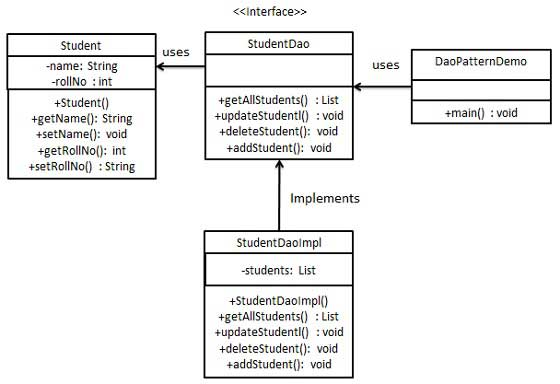
\includegraphics[width=\textwidth]{dao_pattern_uml_diagram.jpg}
        \caption{Esempio di pattern DAO.}
        \source{\href{https://www.tutorialspoint.com/design_pattern/images/dao_pattern_uml_diagram.jpg}{www.tutorialspoint.com}}
      \end{figure}
      \paragraph*{}
      L'esempio sopra mostrato descrive un caso nel quale l'applicazione \emph{DaoPatternDemo} utilizza un oggetto implementante l'interfaccia \emph{StudentDao} per ottenere oggetti (DTO) di tipo \emph{Student}.
      Come il dao recupererà i dati non è rilevante per DaoPatterDemo: si è quindi liberi di modificare l'implementazione di StudentDao.
      \paragraph*{}
      Il progetto però punta a generare dei DAO per oggetti che verranno a loro volta generati in futuro: non è quindi possibile definire DTO e tanto meno interfacce e metodi personalizzati per gestirli.
      Si potrebbero supportare solo operazioni estremamente generiche, come "elenca tutte i record", "elimina tutti i record", "estrai l'n-esimo record"\dots.
      \paragraph*{}
      Per superare questa limitazione, l'azienda ha deciso di sfruttare il supporto che TypeScript offre per i tipi generici: le interfacce della libreria puntano a definire un DAO generico adatto ad ogni tipo di DTO.
      \begin{figure}[H]
        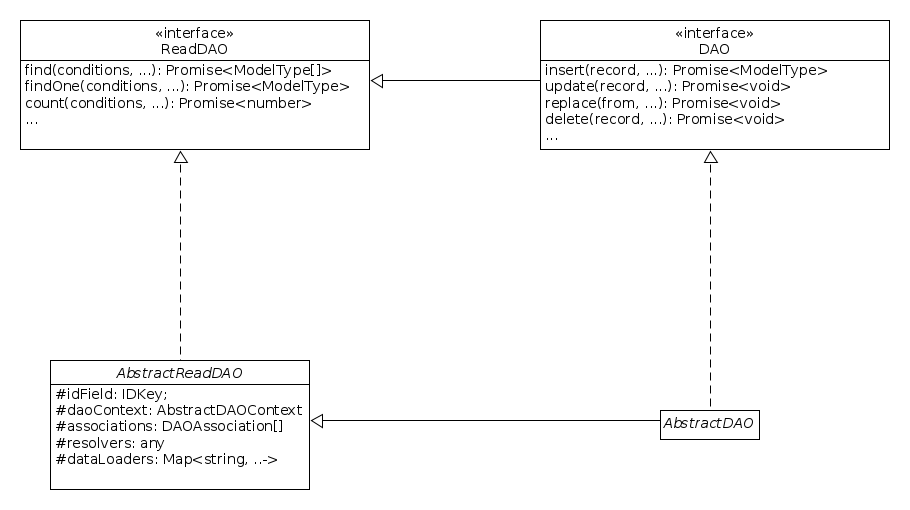
\includegraphics[width=\textwidth]{prototype-architecture.png}
        \caption{Architettura dei principali componenti del prototipo aziendale.}
      \end{figure}
      \paragraph*{}
      L'entità DAO alla base della libreria è l'interfaccia \emph{ReadDAO}: oltre a definire metodi per la ricerca, l'interfaccia specifica anche le firme per quelli che servono a gestire le \emph{associazioni}.
      \paragraph*{}
      Viene infatti definito un meccanismo di associazioni tra DAO indipendente dal database sottostante, così da poter implementare associazioni fra i vari tipi dello schema GraphQL anche in database non relazionali.
      \paragraph*{}
      Le associazioni, oltre all'implementazione dei metodi per gestirle, sono contenute nel classe astratta \emph{AbstractReadDAO}.
      I metodi di lettura invece sono implementati come template methods.
      \paragraph*{}
      La struttura principale delle associazioni fra DAO è la seguente:
      \begin{Verbatim}[samepage=true]
        type DAOAssociation = {
          type: DAOAssociationType,
          reference: DAOAssociationReference,
          field: string,
          refFrom: string,
          refTo: string,
          dao: string,
          ...
        }
      \end{Verbatim}
      \begin{itemize}
        \item I campi \emph{type} e \emph{reference} indicano se l'associazione è di tipo \emph{foreign/inner} e \emph{uno a molti/uno a uno};
        \item \emph{field} indica il nome del campo che andrà risolto come associazione
        \item \emph{refFrom} e refTo sono i nomi dei campi che fungono da chiavi per la relazione
        \item \emph{dao} è il nome del DAO associato
      \end{itemize}
      \paragraph*{}
      Quando un campo con nome uguale al parametro \emph{field} viene ricercato nel DAO che contiene l'associazione, prima viene risolta l'operazione di ricerca sul DAO interrogato, dopodiché
      viene effettuata una lettura anche sul DAO associato al campo \emph{field} tramite il metodo \emph{load}, definito (ma non mostrato nello schema) nell'interfaccia ReadDAO.
      \paragraph*{}
      L'interfaccia \emph{DAO} estende l'interfaccia ReadDAO e completa il set di operazioni aggiungendo la definizione dei metodi di scrittura (insert, update, replace\dots).
      La sua implementazione astratta si limita a definire questi metodi come template methods.
      \paragraph*{}
      I parametri dei metodi di lettura e scrittura sono principalmente tre: \emph{filtri}, \emph{ordinamenti} e \emph{proiezioni}.
      Poiché il DAO deve operare su qualsiasi tipo di DTO, la struttura di questi tre parametri verrà generata durante il processo di generazione del codice e i loro tipi
      verranno passati fra i parametri generici del DAO generato.
      \paragraph*{}
      La classe \emph{AbstractDAO} dovrà essere poi implementata da classi astratte dedicate per ogni tipo di DB sottostante: l'azienda ha già definito ed implementato la classe \emph{AbstractMongooseDAO} per gestire la comunicazione con un database MongoDB.
      \paragraph*{}
      Durante il processo di generazione del codice vengono poi generate varie implementazioni di questa classe astratta, una per ogni DTO da gestire.
      \paragraph*{}
      Ultimo componente della libreria è la classe \emph{AbstractDAOContext}. Questa si occupa principalmente di contenere istanze di tutti i DAO dell'applicazione e di inizializzarli.
      Come mostrato precedentemente nello schema, ogni DAO possiede un riferimento al DAOContext così che, tramite questo, ogni DAO possa comunicare con gli altri (per esempio per risolvere associazioni).
    \section{Requisiti}
      Lo scopo di questa tesi è quello di ampliare le capacità del prototipo aziendale, rendendo possibile generare anche modelli per database SQL.
      Confrontandomi con il referente aziendale, sono stati individuati i seguenti requisiti.
      \subsection{Requisiti funzionali}
        \begin{itemize}
          \item il sistema deve potersi interfacciare con un database SQL, traducendo le query dal formato aziendale a SQL.
          \item il sistema sviluppato deve essere in grado di tradurre uno schema GraphQL in formato tabellare, in particolare:
          \begin{itemize}
            \item deve poter generare tabelle SQL ed opportune relazioni basate sui tipi definiti in uno schema GraphQL. Particolare attenzione viene posta su tipi dalle caratteristiche più complesse, quali:
            \begin{itemize}
              \item tipi con composizioni, nel caso un tipo GraphQL ne comprenda altri fra i suoi campi;
              \item tipi associati ad altri tipi tramite direttive sullo schema GraphQL;
              \item ereditarietà fra interfacce e tipi che le implementano.
            \end{itemize}
            \item deve poter generare DAO per gestire la lettura/scrittura sulle tabelle generate;
            \item deve poter generare tipi di supporto, come filtri, proiezioni e ordinamenti, personalizzati per ogni DAO;
          \end{itemize}
          \item il sistema deve poter supportare tipi di dato personalizzati nei campi dei tipi.
        \end{itemize}
      \subsection{Requisiti non funzionali}
        \begin{itemize}
          \item la comunicazione con il database e la traduzione delle query devono essere implementate utilizzando la libreria Sequelize;
          \item l'interazione con i DAO deve essere quanto più vicina a quella della versione per MongoDB, per non dover modificare la parte comune della libreria;
          \item lo schema GraphQL per generare il codice deve essere quanto più simile a quello per la versione MongoDB. Si possono invece modificare liberamente le direttive aggiuntive usate nello schema;
          \item il sistema non deve creare un overhead eccessivo per la risoluzione delle operazioni.
        \end{itemize}
  \newpage
  
  \chapter{Sviluppo del DAO}
    \paragraph*{}
    Le problematiche maggiori della fase di implementazione del DAO astratto sono scaturite dalle differenze fra database di tipo documentale (come MongoDB) e database SQL.
    Gli schemi GraphQL utilizzati dall'azienda per eseguire test, e che sono stati presi come punto di riferimento per lo sviluppo dell'implementazione, presentano alcuni tipi difficilmente convertibili in formato tabellare, questo perché gli schemi GraphQL sono
    più adatti per definire modelli per database NoSQL.
    \section{Differenze tra database SQL e NoSQL}
    \paragraph*{}
      I database NoSQL non sono basati su tabelle rigidamente definite e associate fra di loro; esistono diversi tipi di schemi per database NoSQL fra cui quelli \emph{documentali}, a \emph{chiave-valore} e basati su \emph{grafi}.
      \paragraph*{}
      In particolare, i database documentali contengono al loro interno \emph{documenti}, strutture dati tipicamente organizzate internamente come serie di chiavi-valori (ad esempio, implentando i formati JSON, XML o YAML).
      A differenza dei database relazionali, tutte le informazioni relative ad un documento sono all'interno della sua istanza e non distribuite fra più tabelle collegate tramite \emph{relazioni}.
      I database documentali (NoSQL, in generale) contengono principalmente dati di tipo non strutturato e i singoli record possono anche omettere completamente campi descritti nel loro schema.
      \begin{figure}[H]
        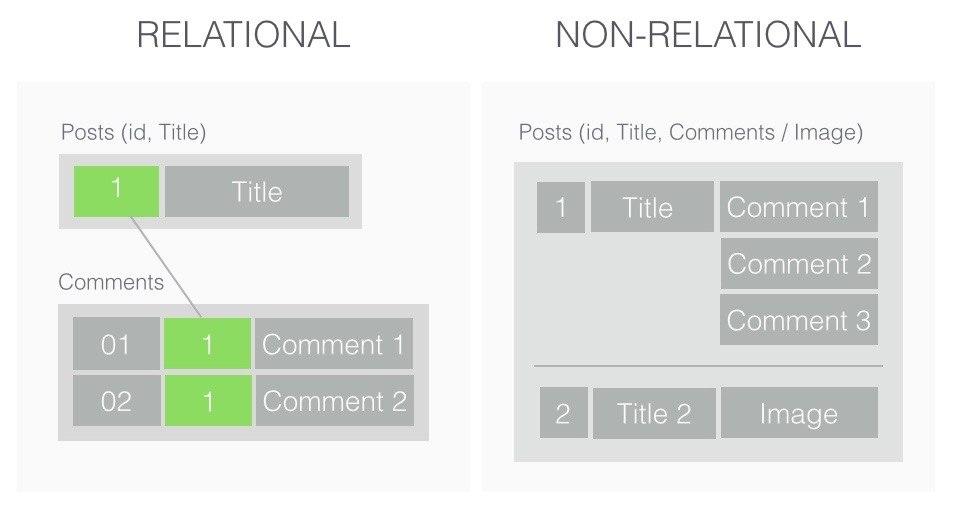
\includegraphics[width=\textwidth]{relational-documental.jpg}
        \caption{Esempio differenze fra schemi SQL e Documenti.}
        \source{\href{https://www.upwork.com/resources/sql-vs-nosql-databases-whats-the-difference/}{www.upwork.com}}
      \end{figure}
    \section{Individuazione di casi problematici}
    \paragraph*{}
    Di seguito è mostrato un esempio di tipo dalla difficile mappatura in un database SQL:
        \hypertarget{tipo-difficile}{}\begin{Verbatim}[samepage=true]
        type Person implements Account {
            id: ID!
            name: String!
            address: Address
            dog: Dog
            amount: Float
            dogSittersId: [ID!]
            dogSitters: [DogSitter!] @mongoInnerRef
            beagleId: ID!
            beagle: Beagle @mongoInnerRef
        }
      \end{Verbatim}
      \paragraph*{}
      I campi seguiti dalla direttiva \emph{@mongoInnerRef} non sono mappati sul database, ma verranno gestiti come associazioni con il meccanismo di associazioni fra DAO.
      \paragraph*{}
      I problemi di tipi come questo sono:
      \begin{itemize}
        \item Il tipo estende un'interfaccia
        \item Al suo interno il tipo contiene un campo di un altro tipo: \emph{Address} (questi tipi non rappresentano tabelle sulle quali effettuare richieste direttamente, ma sono tipi innestati nei tipi delle tabelle)
        \item Al suo interno il tipo contiene un campo di tipo interfaccia: \emph{Dog}
        \item Al suo interno il tipo contiene degli array
      \end{itemize}
      \paragraph*{}
      Database di tipo SQL non hanno soluzioni uniformi fra le varie implementazioni (o non ne hanno per niente) per gestire oggetti innestati, array e gerarchie.
      \paragraph*{}
      Anche l'interazione con i DAO che gestiscono tipi complessi come quello appena segnalato presenta problematiche: è infatti previsto, almeno nella versione mongoose, che si possa interagire con i DAO delle interfacce come se si stessero interrogando anche i DAO delle implementazioni.
      Per esempio, dati i tipi
      \begin{Verbatim}[samepage=true]
        interface User @mongoEntity {
          id: ID! @id
        }
        type CustomerUser implements User {
          id: ID!
          profile: ProfessionalProfile
        }
      \end{Verbatim}
      mappati in tipi TypeScript nel seguente modo
      \begin{Verbatim}[samepage=true]
        export type User = {
          id: Scalars['ID'];
        };
        export type CustomerUser = User & {
          __typename?: 'CustomerUser';
          id: Scalars['ID'];
          profile?: Maybe<ProfessionalProfile>;
        };
      \end{Verbatim}
      dovrebbe essere possibile effettuare la seguente operazione
      \begin{Verbatim}[samepage=true]
        let customerUser : CustomerUser = 
          { id: user.id, __typename: "CustomerUser",
            firstName: "FirstName 1", organizationId: "organization_id",
            live: true };
        await DAO.user.insert(customerUser);
      \end{Verbatim}
      ed aspettarsi, interrogando successivamente il DAO di user, di ricevere in risposta il record di tipo CustomerUser con tutti i suoi attributi, anche quelli non relativi alla tabella degli Users.
    \section{Risoluzione delle problematiche - alto livello}
      In un primo momento era stato ipotizzato di gestire i casi sopra descritti con delle associazioni, sfruttando il meccanismo di riferimenti già presente nel progetto dell'azienda.
      Questo approccio avrebbe però portato a dover gestire una serie di complicazioni:
      \begin{itemize}
        \item Generazione manuale delle tabelle di giunzione per gestire le relazioni fra tipi
        \item Necessità di effettuare modifiche all'interfaccia delle associazioni, quindi dover modificare l'interfaccia del DAO comune
        \item Dipendenza di associazioni l'una dall'altra: è per esempio possibile che un'associazione interna dipenda da un campo contenuto in un oggetto innestato; essendo, nel caso SQL, l'oggetto embedded rappresentato da un'altra tabella associata, sarebbe stato necessario definire un meccanismo per rilevare e gestire le dipendenze fra le due associazioni.
      \end{itemize}
      Sono stati invece evitati questi problemi usando le associazioni di Sequelize.
      \paragraph*{}
      (nota: verrà usato il termine \emph{riferimenti} per riferirsi alle associazioni indicate su schema GraphQL e risolte tramite il meccanismo interno al DAO, mentre \emph{associazioni} per intendere associazioni Sequelize)
      Non usando il meccanismo di gestione dei riferimenti si evita di dover effettuare cambiamenti all'interfaccia comune e non bisogna gestire dipendenze fra essi, in quanto la loro risoluzione verrà eseguita solo dopo che il DAO Sequelize avrà raccolto tutti i dati della tabella e di quelle associate.
      Oltre a questo, Sequelize gestisce in autonomia (o dietro configurazione esplicita) la creazione di foreign keys per collegare le tabelle fra di loro, non rendendo necessario aggiungere questi campi, utili solo alla versione SQL, nello schema GraphQL.
      \paragraph*{}
      I campi di tipi embedded verranno mappati in tabelle secondarie, con riferimenti alle tabelle alle quali appartengono.
      Gli array vengono gestiti tramite l'associazione Sequelize di tipo HasMany: nel caso siano array di dati scalari, verrà creata una tabella apposita per contenere questi valori.
      \paragraph*{}
      Per la gestione delle interfacce è stato scelto di tenere tutti i campi comuni in una tabella relativa all'interfaccia, mentre in quelle delle implementazioni saranno salvati i dati relativi ad esse ed un riferimento al record associato sulla/e tabella/e dell'interfaccia/e.
      Viene aggiunto, dove non indicato nello schema GraphQL, un campo id fittizio.
      Per gestire le tabelle aggiuntive verranno inizializzati dei DAO dedicati, tenendoli però nascosti all'utilizzatore dell'applicazione.
      \paragraph*{}
      Il tipo \hyperlink{tipo-difficile}{precedentemente mostrato} e quelli associati verranno quindi mappati con la seguente struttura di tabelle
      \begin{figure}[H]
        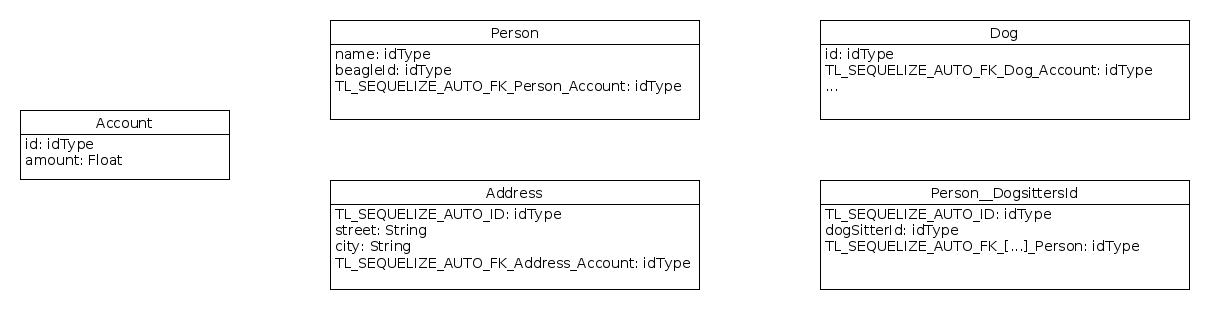
\includegraphics[width=\textwidth]{db-example.jpg}
        \caption{Schema delle tabelle per l'entità \emph{Person}}
      \end{figure}
      \paragraph*{}
      I campi aggiuntivi sono quelli con la dicitura \emph{TL_SEQUELIZE_AUTO} mentre Person_dogSittersId è una tabella aggiunta che serve per contenere i valori dell'array \emph{dogSittersId}.
      \paragraph*{}
      Per gestire le associazioni fra DAO è stata definita la seguente interfaccia:
      \begin{Verbatim}[samepage=true]
        interface SequelizeAssociation {
          field : string,
          daoModelName : string,
          kind : SequelizeAssociationKind
          alias: string,
          extractField? : string,
        }
      \end{Verbatim}
      \paragraph*{}
      Ogni DAO conserva una mappa che, al nome di un campo, associa una tupla composta dal DAO associato a quel campo e dalla SequelizeAssociation corrispondente.
      Il significato dei campi è il seguente:
      \begin{itemize}
        \item field: nome del campo associato ad un altro DAO
        \item daoModelName: nome del DAO associato
        \item kind: indica se il DAO associato rappresenta un tipo \emph{embedded}, \emph{interfaccia} o \emph{implementazione}
        \item alias: alias dell'associazione SQL fra i modelli dei DAO
        \item extractField: opzionale. Se utilizzato in un'associazione di tipo embedded, indica che il/i model associati dovranno essere mappati al campo indicato.
                            Nell'applicazione, verrà usato per gestire gli array di primitive.
      \end{itemize}
      Il principio di funzionamento generale dell'applicazione è quindi quello di rilevare quando un campo presente nei parametri della query è relativo ad un DAO associato e, di conseguenza, delegare la risoluzione di quel campo al DAO.
      \paragraph*{}
      Per impedire modifiche parziali, le operazioni di modifica (inserimento, aggiornamento, rimozione) saranno effettuate all'interno di \emph{transazioni} SQL.
      Se per esempio si verificasse un problema nell'inserimento di una sottoclasse, la parte di record contenuta nella tabella della superclasse non dovrebbe venire salvata.
    \section{Risoluzione delle problematiche - implementazione}
      Le funzioni principali del DAO astratto da implementare sono:
      \begin{itemize}
        \item Insert - Inserimento.
        \item Find   - Ricerca
        \item Update - Aggiornamento
        \item Delete - Eliminazione
      \end{itemize}
      Tutte le altre operazioni (come \emph{count} e \emph{replace}) sono derivabili da queste.
      \paragraph*{}
      Per gestire le associazioni, molti dei metodi scritti hanno una struttura ricorsiva del tipo:
      \begin{Verbatim}[samepage=true]
        function recursiveFunction(query, ...) {
          for(let field in query) {
            const a = this.sequelizeAssociations.get(field)
            if (a) {
              if(a is of kind EMBEDDED) {
                a.getDao().recursiveFunction(query[field])
              } else {
                a.getDao().recursiveFunction({field : query[field]})
              }
            }
            ...
          }
        }
      \end{Verbatim}
      Se un'associazione viene rilevata su un campo del parametro query, la funzione verrà richiamata sul DAO associato a quel campo. 
      Bisogna però fare attenzione al tipo di associazione: se è di tipo embedded, il DAO associato si occuperà di gestire direttamente il dato passato. Altrimenti, vuol dire che il DAO associato è una interfaccia o implementazione e potrebbe dover
      delegare nuovamente il campo ad un DAO associato in modo embedded.
    \subsection{Inserimento}
      Per l'inserimento è definita una sola funzione, che accetta il record da inserire nel database ed eventuali opzioni di scrittura.
      Sequelize permette di effettuare l'operazione di inserimento passando direttamente un oggetto composto, a patto di includere le associazioni alle tabelle relative
      nel parametro "options" di input.
      \paragraph*{}
      Esempio di inserimento di un oggetto di tipo Product, uno User associato e indirizzi associati allo user.
      \begin{Verbatim}[samepage=true]
        return Product.create({
            title: 'Chair',
            user: {
                firstName: 'Mick',
                addresses: [{
                    city: 'Austin',
                },{
                    city: 'New York',
                }]
            }
            }, {
            include: [{
                association: Product.User,
                include: [ User.Addresses ]
            }]
        });
      \end{Verbatim}
      \paragraph*{}
      L'inserimento viene quindi eseguito in due fasi:
      Nella prima, il record passato in input viene processato e tutti i suoi campi associati vengono raggruppati dietro all'\emph{alias} delle associazioni.
      Nel caso dell'esempio precedente, in un oggetto di tipo
      \begin{Verbatim}[samepage=true]
        {
          title: 'Chair', 
          firstName: 'Mick',
          addresses: [{city: 'Austin}, ...]
        }
      \end{Verbatim}
      passato come input al DAO "product", vengono rilevate le associazioni ai campi "firstName" e "addresses" e raggruppate dietro l'alias ("user") dell'associazione, come mostrato nell'esempio sopra.
      Ricorsivamente, nel DAO "user", viene gestito il campo associato "addresses".
      \paragraph*{}
      Nella seconda fase viene invece costruito l'oggetto delle opzioni che deve ricorsivamente indicare tutte le associazione incluse nella query.
    \subsection{Ricerca}
      \subsubsection*{Interfaccia della funzione Sequelize}
        Sequelize permette di effettuare un'operazione di ricerca includendo subito uno o più modelli associati, tramite il meccanismo di Eager Loading.
        \paragraph*{}
        Esempio di semplice query di ricerca con un modello associato, nella quale viene indicato anche l'alias dell'associazione:
        \begin{Verbatim}[samepage=true]
          const users = await User.findAll({
            include: { model: Tool, as: 'instruments' }
          });
        \end{Verbatim}
        \paragraph*{}
        È possibile, in alternativa al passare la coppia di attributi "model"/"as", definire un campo "association", inizializzato con il nome dell'associazione.
        \begin{Verbatim}[samepage=true]
          User.findAll({ include: { association: 'instruments' } });
        \end{Verbatim}
        \paragraph*{}
        È anche supportata l'inclusione di più modelli alla volta, nonché di modelli associati a quelli inclusi, in modo innestato.
        \begin{Verbatim}[samepage=true]
          User.findAll({ 
            include: [
              { association: 'instruments' }, 
              { association: 'Tools', 
                include : [
                  association : 'Designers'
                ]
              }
            ]
          });
        \end{Verbatim}
        \paragraph*{}
        Tramite l'opzione \emph{where} è invece possibile definire un filtro per la ricerca.
        \begin{Verbatim}[samepage=true]
          User.findAll({
            where : {firstName : 'Paul'},
            include: {
              association: 'instruments',
              where: {
                size: {
                  [Op.ne]: 'small'
                }
              }
            }
          });
        \end{Verbatim}
        \paragraph*{}
        Definire così le opzioni di ricerca scollegherebbe i filtri dei campi di una tabella da quelli dei campi di una tabella che rappresenterebbe un oggetto innestato in quella precedente.
        Ad esempio, supponendo che l'associazione "instruments" rappresenti un oggetto embedded in User, il filtro di ricerca
        \begin{Verbatim}[samepage=true]
          userFilter : UserFilter = {
            $or : {
              firstName : 'Paul', 
              "instruments.size" : {
                $ne : 'small'
              }
          }}
        \end{Verbatim}
        Non sarebbe traducibile, non potendo mettere in "OR" i due filtri, secondo la modalità precedente presentata.
        \paragraph*{} 
        Fortunatamente, Sequelize permette di elevare allo stesso livello tutti i filtri, risolvendo così il problema.
        \begin{Verbatim}[samepage=true]
          User.findAll({
            where : {
              [Op.or] : {
                "$firstName$" : 'Paul', 
                "$instruments.size$" : {
                  [Op.ne] : 'small'
                }
              }
            },
            include: {
              model: Tool,
              as: 'instruments'
            }
          });
        \end{Verbatim}
        \paragraph*{}
        È possibile indicare, per ogni modello incluso, una lista di attributi da estrarre. Grazie a questo è possibile implementare la proiezione di attributi.
        \paragraph*{}
        L'ordinamento, similmente ai filtri, è specificabile sia modello per modello che al livello radice della query. Quest'ultima opzione è stata scelta.
        Ad esempio, l'ordinamento
        \begin{Verbatim}[samepage=true]
          userSort : UserSort = [
            {firstName : SortDirection.ASC},
            {"instruments.size" : SortDirection.DESC}
          ]
        \end{Verbatim}
        può essere tradotto in una query Sequelize nel seguente modo:
        \begin{Verbatim}[samepage=true]
          User.findAll(
            {
              order: [
                ['firstName', 'ASC'],
                ['instruments', 'size', 'DESC']
              ]
              include: {
                model: Tool,
                as: 'instruments'
              }
            });
        \end{Verbatim}
      \subsubsection*{Gestione delle inclusioni}
        Sequelize permetterebbe di effettuare automaticamente un join fra il Model iniziale, tutti quelli associati e potenzialmente anche quelli associati a quelli associati tramite l'opzione, da inserire nella query,
        \emph{attributes: \{all : true, nested : true\}}.
        \paragraph*{}
        Questo semplificherebbe di molto il problema della gestione della query, ma ogni interrogazione comporterebbe un numero elevato di operazioni di join.
        Per ridurre il numero di join l'implementazione cercherà di includere solo le tabelle strettamente necessarie.
        \paragraph*{}
        A tal proposito vengono analizzati filtri, proiezioni e ordinamenti ricevuti in input per identificare i modelli da includere nella ricerca.
        Per fare ciò, i parametri in input vengono tradotti, dove serve, sia in un formato comprensibile per Sequelize, sia in un oggetto a più livelli per facilitare l'individuazione di campi associati.
        \paragraph*{}
        Per esempio, il filtro "userFilter" precedentemente mostrato viene convertito in
        \begin{Verbatim}[samepage=true]
          {
            $or : {
              firstName : 'Paul',
              instruments : {
                size : {
                  $ne : 'small'
                }
              }
            }
          }
        \end{Verbatim}
        così da poter, rilevare, percorrendo ricorsivamente la struttura, l'associazione con il model Tool sul campo instruments.
    \subsection{Aggiornamento}
      Sono rese disponibili tre funzioni di aggiornamento: 
      \begin{itemize}
        \item update: accetta un oggetto di tipo ModelType, cerca di individuarlo nel database ed aggiornarlo
        \item updateOne: accetta un filtro di ModelType e aggiorna il primo record individuato in base ad esso
        \item updateMany: accetta un filtro di ModelType e aggiorna tutti i record individuati in base ad esso
      \end{itemize} 
      Tutte e tre le funzioni ricevono anche in input un oggetto per definire gli aggiornamenti da scrivere.
      \paragraph*{}
      L'operazione di aggiornamento con modelli associati non è correntemente supportata da Sequelize, quindi è stato implementata una funzione ricorsiva che, dati in input i modelli da aggiornare e i cambiamenti da apportare, esegue il seguente procedimento:
      \begin{enumerate}
        \item per ogni campo dell'oggetto che indica gli aggiornamenti, si controlla se il nome di questo campo corrisponde a quello di un'associazione;
        \begin{enumerate}
          \item in caso positivo, per ogni istanza di model nella tabella corrente si controlla se il dato passato come aggiornamento è un array;
          \begin{itemize}
            \item nel caso lo sia, tutti i modelli associati al modello in esame tramite quel campo devono essere eliminati e sostiuiti con quelli in ingresso: gli id degli elementi da eliminare vengono salvati in una lista, poi vengono inseriti e associati gli elementi del nuovo array.
            \item altrimenti, se esistono, i model associati a quel campo sono da aggiornare ricorsivamente. Vengono salvati in una lista;
            \item in caso non esistano, vengono inseriti;
          \end{itemize}
          \item viene eseguita l'eliminazione in blocco di tutti i model salvati nell'apposita lista, poi si richiama ricorsivamente la funzione di aggiornamento passando come parametri la lista dei modelli associati da aggiornare e i cambiamenti a loro relativi;
        \end{enumerate}
        \item alla fine, vengono mappati tutti i modelli da aggiornare ai loro id, per poter eseguire un'unica operazione di aggiornamento in blocco sulla tabella sfruttando come filtro la lista di id, piuttosto che chiamare la funzione di aggiornamento per ogni modello (effettuando quindi n operazioni di update);
      \end{enumerate}
      I modelli passati alla prima invocazione della funzione sono ottenuti eseguendo un'operazione di ricerca.
    \subsection{Eliminazione}
      Le funzioni di eliminazione da implementare sono due:
      \begin{itemize}
        \item deleteOne: funzione che riceve in input un oggetto e cerca di eliminare il record equivalente nel database
        \item deleteMany: funzione che riceve in input un filtro e cerca di eliminare tutti i record del database che lo soddisfano
      \end{itemize}
      \paragraph*{}
      L'eliminazione di un modello e di tutte le sue associazioni di tipo hasOne/hasMany è gestita automaticamente da Sequelize impostando nell'associazione l'opzione sql ONDELETE CASCADE.
      Questo però non copre due casi: quello in cui si chiami la funzione di eliminazione sul DAO di una implementazione e quello in cui lo si chiami su quello di una interfaccia la quale implementazione implementa due o più interfacce.
      \paragraph*{}
      Nel primo caso verrebbe eliminato solo il record dell'implementazione mentre quelli relativi alle interfacce no, poiché associati con associazioni di tipo "belongsTo", mentre nel secondo il record dell'interfaccia e dell'implementazione verrebbero eliminati, ma quelli delle altre interfacce no, non essendo associati alla prima.
      \paragraph*{}
      Visto che solo i record delle implementazioni conoscono tutte le interfacce ad essi collegati, sono i DAO di questi a gestire le operazioni di eliminazione: se la funzione viene chiamata sul DAO di un'interfaccia, questo la rigira a tutti i DAO rilevanti di implementazioni.
      I DAO delle implementazioni poi si occuperanno di distruggere i record corretti sui modelli delle interfacce.
      \paragraph*{}
      La funzione delete dei model della libreria Sequelize accetta fra i parametri un filtro per indicare quali record andranno eliminati, ma non permette di includere nel filtro campi di altre tabelle (come nel caso della ricerca).
      Nel caso dell'operazione deleteMany quindi, sarà prima necessario recuperare tutti i model da eliminare con una ricerca per poi mapparli sui loro id, così da rendere il filtro per l'operazione di delete corretto, lo stesso procedimento viene effettuato anche sulle interfacce.
    \newpage
    \chapter{Sviluppo del generatore}
      Il sistema per la generazione dei modelli è stato suddiviso, seguendo la struttura già adottata dall'azienda, nei seguenti moduli:
      \begin{itemize}
        \item Un plugin per GraphQL-code-generator per tenere in comunicazione gli altri moduli
        \item Un file per gestire il trattamento dei nodi del modello GraphQL (implementando il pattern visitor)
        \item Un generatore per verificare la validità dei nodi e invocare metodi di generazione
        \item Un generatore astratto per contenere metodi comuni e le sue implementazioni:
        \begin{itemize}
          \item Un generatore per generare gli schemi Sequelize
          \item Un generatore per generare DAO e tipi di supporto
        \end{itemize}
      \end{itemize}
      \begin{figure}[H]
        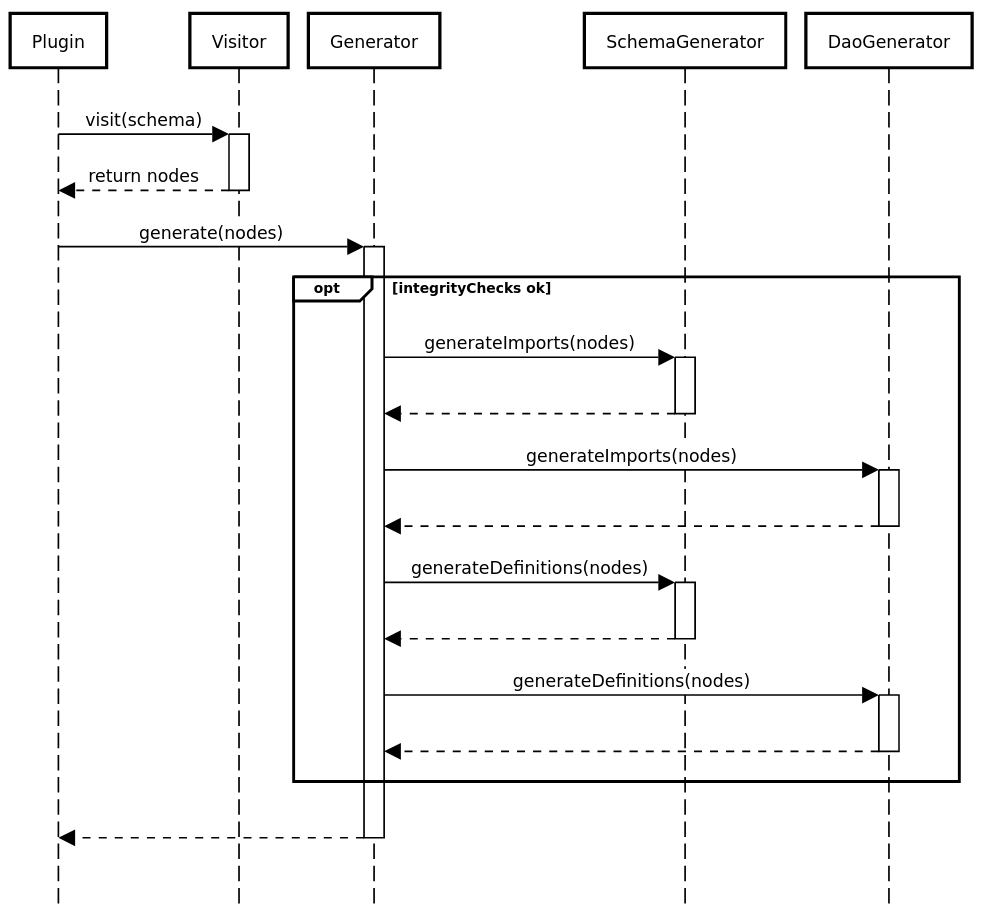
\includegraphics[width=\textwidth]{generator_workflow.png}
        \caption{Flusso di comunicazione fra i vari moduli del generatore}
      \end{figure}
      \paragraph*{Modulo visitor}
      Viene definito un oggetto che estende la classe \emph{BaseVisitor} di GraphQL-codegen ed implementa metodi \emph{visit} per gestire definizioni di tipi ed interfacce.
      Nodi interfaccia e tipo vengono trattati in modo simile e il loro trattamento genera uno o più oggetti (nel caso sia necessario creare tabelle di supporto per quella principale) di tipo \emph{TsSequelizeGeneratorNode}.
      \begin{Verbatim}[samepage=true]
        export enum NodeTypes {
          INTERFACE,
          TYPE,
          EMBEDDED
        }
        export type TsSequelizeGeneratorNode = {
          type?: NodeTypes
          name: string
          isAutoGenerated: boolean
          collection: string
          interfaces: string[]
          fields: TsSequelizeGeneratorField[]
          ...
        }       
      \end{Verbatim}
      Campi principali del tipo TsSequelizeGeneratorNode:
      \begin{itemize}
        \item type: è assente se il nodo è autogenerato (vedere in seguito), altrimenti prende uno dei valori dell'enum NodeTypes.
        \item name: nome del nodo
        \item isAutoGenerated: identifica se il nodo è stato aggiunto pur non essendo presente nello schema GraphQL. Nell'implementazione attuale, questo è il caso dei nodi creati per gestire array di dati primitivi.
        \item collection: nome della tabella nel database
        \item interfaces: nome delle interfacce del nodo
        \item fields: collezione contenente i campi del nodo trattato
      \end{itemize}
      \paragraph*{Modulo generatore}
      Il modulo di generazione, invocato dal plugin dopo aver raccolto tutti i nodi trattati, analizza ognuno di questi e ne controlla la correttezza.
      In particolare, viene verificato che:
      \begin{itemize}
        \item Ogni nodo abbia un campo id o almeno una interfaccia con un campo tale.
        \item I campi sui quali i riferimenti (segnalati tramite direttiva @sqlizeForeignRef o @sqlizeInnerRef) si basano siano esistenti.
        \item I campi condivisi fra implementazioni ed interfacce siano di tipo compatibile.
      \end{itemize}
      \paragraph*{}
      Dentro la classe del generatore è contenuta una lista di implementazioni di generatore del file finale, tutti implementanti una classe astratta.
      Dopo aver controllato tutti i punti precedenti, il generatore principale invoca i metodi di generazione di imports, definizioni ed exports dei generatori della lista.
      \paragraph*{Generatore degli schemi db}
      Il generatore degli schemi di Sequelize analizza tutti i nodi, generando per ciascuno un model Sequelize.
      Gli attributi del model generato corrispondono ai campi del nodo che:
      \begin{itemize}
        \item Non hanno direttive di tipo "reference" nello schema
        \item Non appartengono ad interfacce
        \item Non sono etichettati come liste
        \item Non sono etichettati come di tipo embedded
      \end{itemize}
      \paragraph*{Generatore dei DAO}
      Per ogni nodo generato dal visitor, il generatore dei DAO verifica in primo luogo se l'attributo "isAutoGenerated" è impostato.
      Nel caso lo sia, significa che il nodo non è parte dello schema GraphQL e che quindi il plugin di generazione dei tipi TypeScript, lanciato prima del plugin personalizzato descritto in queste sezioni, non ha generato un tipo relativo ad esso.
      Il generatore dei DAO deve quindi definire tipi per gestire i nodi autogenerati poiché gli oggetti di tipo SequelizeAbstractDAO richiedono fra i parametri generici anche il tipo del DTO.
      \paragraph*{}
      Il generatore dei DAO si occupa anche, per ogni nodo, di generare filtri, proiezioni e ordinamenti sulla base dei campi del nodo.
      \paragraph*{}
      Infine, per ogni nodo, genera l'oggetto di tipo DAO, inizializzandolo con i corretti riferimenti e sequelizeAssociations.
      \paragraph*{}
      Dopo aver generato tutti i DAO, il generatore definisce anche il DaoContext, oggetto che inizializza i DAO e ne contiene un riferimento.
      È il DaoContext che, ricevuta in input un'istanza di oggetto Sequelize, inizializza tutti i modelli definiti dal generatore degli schemi e le loro associazioni Sequelize. 
    \newpage
    \chapter{Valutazione dei risultati}
      \section{Testing}
        Una volta superate le fasi di studio iniziale e prodotto un primo prototipo, parte del processo di sviluppo dei tools e del DAO astratto è stato dedicata al testing.
        \paragraph*{}
          A tal scopo, è stato definito manualmente un ambiente di prova che simulasse un possibile output finale finale del generatore.
          In particolare, è stata prestata attenzione alla creazione di tipi che potessero essere usati per testare alcuni punti critici:
          \begin{itemize}
            \item tipi con tipi embedded fra i loro campi;
            \item tipi con tipi embedded fra i loro campi, a loro volta composti da altri tipi innestati;
            \item tipi con array, sia di primitive che di tipi, fra i loro campi;
            \item tipi che estendono una interfaccia;
            \item tipi che estendono più interfacce;
            \item interfacce estese da più tipi;
          \end{itemize}
        \paragraph*{}
          Per questo ambiente sono stati poi scritti una serie di \emph{unit tests}, utilizzando la libreria di testing JavaScript \emph{Jest}, già impiegata nelle prove del prototipo aziendale vista la sua semplicità di utilizzo ed integrazione.
        \paragraph*{}
          Questi test sono stati scritti per verificare il comportamento delle operazioni del DAO sia in caso di manipolazioni di dati di tipo semplice, sia in caso di tipi più complessi, come quelli elencati precedentemente.
          Vengono di seguito illustrati i casi più interessanti, anche per dimostrare il funzionamento del prodotto della tesi.
          \paragraph*{}
          Gli esempi seguenti interagiranno con i DAO \emph{user}, \emph{user2} e \emph{subUser}: il primo definisce una interfaccia con gli attributi \emph{firstName}, \emph{a} e \emph{b}, il secondo ha l'attributo \emph{firstName2} mentre subUser è un tipo che implementa le due interfacce e aggiunge l'attributo \emph{subAttr}.
          \begin{Verbatim}[samepage=true]
            type User = {
                id?: Scalars['ID'];
                a?: Maybe<A>;
                b?: Maybe<Array<Scalars["String"]>>;
                firstName?: Maybe<Scalars['String']>;
            };
          \end{Verbatim}
          \begin{Verbatim}[samepage=true]
            type User2 = {
              id?: Scalars['ID'];
              firstName2?: Maybe<Scalars['String']>;
            };
          \end{Verbatim}
          \begin{Verbatim}[samepage=true]
            type SubUser = {
              id?: Scalars['ID'];
              a?: Maybe<A>;
              b?: Maybe<Array<Scalars["String"]>>;
              firstName?: Maybe<Scalars['String']>;
              firstName2?: Maybe<Scalars['String']>;
              __typename? : "SubUser";
              subAttrib?: Maybe<String>
            };

          \end{Verbatim}
        \subsection{Inserimento}
          \subsubsection{Entità innestate e array}
            \begin{Verbatim}
              const record = {
                              firstName: "FirstName",
                              a : { 
                                    a : "A",
                                    a2 : "A2",
                                    d: { 
                                        d : "D",
                                        e : ["E"]
                                       }
                                  },
                              b: ["B1", "B2", "B3"]
                             })
              const user = await dao.user.insert(record);
              expect(user.a).toBeDefined();
              expect(user.a?.a).toBe("A");
              expect(user.a?.d?.d).toBe("D");
              expect(user.a?.d?.e).toHaveLength(1);
              expect(user.b).toBeDefined();
              expect(user.b).toHaveLength(3);
            \end{Verbatim}
            Al metodo \emph{insert} di un DAO viene passato un oggetto composto da:
            \begin{itemize}
              \item campi di tipo scalare;
              \item campi di tipo oggetto;
              \item campi di tipo array.
            \end{itemize}
            Fra i campi di tipo oggetto ce ne sono anche alcuni a loro volta composti da oggetti.
            Si verifica, dopo l'inserimento, che tutti i campi siano esistenti e corretti.
          \subsubsection{Sottoclassi}
            \begin{Verbatim}
              const record = { 
                               firstName: "FirstName",
                               subAttrib: "subAttr"
                             }
              await dao.subUser.insert(record);
              const user = await dao.user.findOne({});
              const subUser = await dao.subUser.findOne({});
              expect(subUser!.firstName).toBe(user!.firstName);
              expect(subUser!.id).toBe(user!.id);
              expect(subUser!.subAttrib).toBe("subAttr");
            \end{Verbatim}
            Si chiama il metodo di inserimento del DAO di SubUser. Si verifica successivamente che sia possibile recuperare lo stesso record inserito sia interrogando il DAO dell'interfaccia che quello dell'implementazione. La prova di uguaglianza fra il record ottenuto dal DAO
            dell'interfaccia e quello dell'implementazione viene fatta su una serie di attributi, fra cui l'ID.
          \paragraph{Classe con più interfacce}
            \begin{Verbatim}
              let su : SubUser = {
                                  firstName : "subName",
                                  firstName2 : "fname2",
                                  subAttrib : "subAttr",
                                  b: ["b1", "b2"]
                                 }
              su = await dao.subUser.insert(su);
              const u = await dao.user.findOne({});
              const u2 = await dao.user2.findOne({});
              expect(su.id).toBe(u?.id);
              expect(su.id).toBe(u2?.id);
            \end{Verbatim}
            Viene inserito un record tramite il DAO di SubUser, che implementa più di una interfaccia. Successivamente si controlla che interrogare il DAO utilizzato o quello delle sue interfacce porti a recuperare lo stesso record.
        \subsection{Aggiornamento}
          \paragraph{Aggiornamento di entità innestate}
            \begin{Verbatim}
              \\[...] inserimento record
              dao.user.updateMany({
                                   "a.d.d" : "D",      //Filtro
                                   "a.d.e" : null
                                  }, {
                                   "a.d.d" : "Dc",     //Aggiornamenti
                                   "a.a" : "A11",
                                   "a.d.e" : "E2",
                                   "b": ["a", "b"]
                                  });
            \end{Verbatim}
            \begin{Verbatim}
              const numUpdated = await dao.user
                                          .count({
                                            "a.d.d" : "Dc",
                                            "a.a" : "A11",
                                            "a.d.e" : "E2",
                                            b : ["a", "b"]
                                          })
              expect(numUpdated).toBe(2)
            \end{Verbatim}
            Vengono inseriti dei record con oggetti innestati e array e poi, sempre sullo lo stesso DAO dell'inserimento, viene chiamata la funzione di aggiornamento, indicando che si vogliono aggiornare solo alcuni dei record aggiunti utilizzando il parametro di tipo filtro.
            I cambiamenti indicati vanno a definire aggiornamenti sia su array che su oggetti, incluso l'aggiornamento di parametri di oggetti innestati dentro oggetti innestati.
            Successivamente si contano i record che sono stati correttamente aggiornati.
          \paragraph{Aggiornamento di sottoclassi}
            \begin{Verbatim}
              let user = await dao.subUser
                                  .insert({ firstName: "FirstName" });
              user = (await dao.subUser.findOne({ id: user.id }));
              await dao.subUser.update(user, { 
                                              subAttrib : "subAttrib",
                                              firstName: "FirstName1"
                                             });
              const user2 = await dao.subUser.findOne({ id: user.id });
              expect(user2!.firstName).toBe("FirstName1");
              expect(user2!.subAttrib).toBe("subAttrib");
            \end{Verbatim}
            Viene inserito un record di tipo SubUser e poi lo si aggiorna.
            Fra i campi aggiornati ce ne sono anche di appartenenti all'interfaccia implementata dal record.
        \subsection{Sostituzione}
          \paragraph{Sostituzione di superclasse con sottoclassi}
            \begin{Verbatim}
              let user = await dao.user
                                  .insert({ firstName: "FirstName" });
              let subUser : SubUser = { 
                                        id: user.id,
                                        firstName: "FirstName 1",
                                        subAttrib: "subAttrib"
                                      };
              await dao.user.replace(user, subUser);
              user = await dao.user.findOne({ id: user.id });
              expect(user).toBeDefined();
              expect(user?.firstName).toBe("FirstName 1");

              \\[...] definizione type guard isSubUser
          
              if(isSubUser(user)){
                  expect(user.subAttrib).toBe("subAttrib");
              } else {
                  fail("Replaced user is not of expected subclass.")
              }
            \end{Verbatim}
            Viene inserito un record tramite il DAO della superclasse, poi sostituito con un oggetto di tipo SubUser.
            Dopodiché, tramite una ricerca per ID, si accede al nuovo record e ne si controlla il tipo, che deve quindi essere diventato quello di SubUser.
        \subsection{Eliminazione}
          \paragraph{Eliminazione di classe con più superclassi}
            \begin{Verbatim}
              const su : SubUser = {
                                    firstName : "subName",
                                    firstName2 : "fname2",
                                    subAttrib : "subAttr"
                                   }
              \\[...] inserimento record
              await dao.subUser.deleteMany({
                                            firstName : "subName",
                                            subAttrib : "subAttr"
                                           })
              expect(await dao.user2.count({})).toBe(0)
            \end{Verbatim}
            Vengono inseriti record di tipo SubUser e successivamente li si eliminano chiamando la funzione di eliminazione sullo stesso DAO.
            Fra i parametri del filtro di eliminazione sono inseriti anche attributi appartenenti ad una delle due interfacce.
            Si verifica poi, tramite una ricerca sul dao della seconda interfaccia, che siano stati correttamente eliminati tutti i record.
      \section{Limiti dell'implementazione proposta}
        Le associazioni salvate nella lista "sequelizeAssociations" di un Dao sono identificate solo tramite il nome di un campo, pertanto non è possibile gestire il caso in cui un DAO abbia più relazioni basate su campi con lo stesso nome.
        È questo per esempio il caso di una interfaccia implementata da due implementazioni (o viceversa) che condividono un campo dal nome uguale ma non presente nell'interfaccia: il DAO dell'interfaccia potrà avere una sola sequelizeAssociation basata sul campo condiviso dalle due interfacce.
        \paragraph*{}
        Viene mostrato un esempio di inserimento nel quale questo problema si manifesta:
        \begin{Verbatim}[samepage=true]
          interface Account {
            id: ID! @id
            amount: Float
            address: Address
            dog: Dog @sqlizeForeignRef(refFrom: "accountId")
          }
        \end{Verbatim}
        \begin{Verbatim}[samepage=true]
          type Person implements Account {
            id: ID!
            amount: Float
            address: Address
            dog: Dog
            name: String!
            surname: String!
          }
        \end{Verbatim}
        \begin{Verbatim}[samepage=true]
          type Business implements Account {
            id: ID!
            amount: Float
            address: Address
            dog: Dog
            name: String!
            vatNumber: String!
          }
        \end{Verbatim}
        \paragraph*{}
        I due tipi che implementano l'interfaccia "Account" hanno entrambi un campo con lo stesso nome ma non appartenente all'interfaccia: "name".
        Il DAO del tipo "Person" verrà generato e inizializzato per primo, dunque "Account" avrà una sequelizeAssociation basata sul campo "name" e collegata con il DAO "Account".
        \paragraph*{}
        Se successivamente si provasse ad inserire un record di tipo "Business" chiamando il metodo di inserimento sul DAO di "Account", quest'ultimo cercherebbe di inserire due record: uno nella tabella "Business" contenente l'attributo "vatNumber" e uno nella tabella "Person" composto dall'attributo "name".
        \paragraph*{}
        Questa limitazione è dovuta all'utilizzo, nel progetto originale, di tipi TypeScript piuttosto che di classi: non potendo riconoscere il tipo dell'oggetto passato in input se non analizzando i suoi campi, collisioni di questo tipo sono difficilmente gestibili.
        \paragraph*{}
        I tipi TypeScript generati dal plugin ufficiale di GraphQL-codegen hanno un campo nominato "__typeName", contente il nome del tipo concreto (quindi non delle interfacce), con il quale si potrebbe risolvere il problema.
        Nella configurazione usata dall'azienda però questo campo è reso opzionale, pertanto un utente potrebbe inserire un record senza specificare il tipo dell'oggetto passato in input.
        \paragraph*{}
        Dopo averne discusso con il referente aziendale, questi limiti non sono stati ritenuti particolarmente preoccupanti, in quanto sono state rilevate problematiche simili anche per la versione MongoDB.
    \newpage
    \chapter{Conclusioni}
      \section*{Risultati}
      In questa tesi sono stati raggiunti gli obiettivi di base concordati con l'azienda: sono state estese le opzioni di generazione di codice del prototipo aziendale rendendolo capace di generare modelli e DAO per un database SQL partendo da uno schema GraphQL.
      \paragraph*{}
      È stata anche sviluppata una prima versione del DAO astratto, in grado di convertire le richieste in formato SQL.
      Tutto il sistema è stato testato sugli stessi (o simili) test della versione originale, con qualche casistica rilevante aggiunta.
      \paragraph*{}
        È stata data considerazione alle prestazioni, cercando di eseguire dove possibile meno operazioni di JOIN per le operazioni di lettura e, per quelle di scrittura, più operazioni di scrittura in blocco.
      \paragraph*{}
        La comunicazione con l'azienda è stata chiara e utile per dissipare eventuali dubbi sulla struttura del progetto o su certi aspetti di MongoDB, database del quale il sottoscritto non ha esperienza.
      \section*{Lavori futuri}
        Oltre ad un supporto continuato (tutto il progetto, comprese le interfacce del DAO, è ancora in fase prototipale), una funzionalità immediatamente aggiungibile sarebbe quella di poter far scegliere, in fase di generazione, come trattare le gerarchie di interfacce e implementazioni.
        Correntemente è possibile gestire le gerarchie solo nel modo descritto nei capitoli precedenti, ma l'azienda sarebbe interessata a poter gestire le gerarchie anche nelle altre due modalità rimanenti:
        \begin{itemize}
          \item accorpando tutte le implementazioni nella tabella dell'interfaccia;
          \item generando solo le tabelle delle implementazioni, ognuna contenente anche i campi delle interfacce;
        \end{itemize}
    \newpage
    \begin{thebibliography}{3}
      \addcontentsline{toc}{chapter}{Bibliografia}
      \bibitem{GraqlQLDoc}GraphQL official site,\\\href{https://graphql.org/learn/}{https://graphql.org/learn/}
      \bibitem{GraphQL-codegenDoc}GraphQL code generator official site,\\\href{https://graphql-code-generator.com/docs/getting-started/index}{https://graphql-code-generator.com/docs/getting-started/index}
      \bibitem{SequelizeAPI}Sequelize documentation,\\\href{https://sequelize.org/master/}{https://sequelize.org/master/}
      \bibitem{MDP}Bran Selic,\\\href{https://www.researchgate.net/publication/221249899_Model-Driven_Development_Its_Essence_and_Opportunities}{Model-Driven Development: Its Essence and Opportunities}
      \bibitem{GraphQL-history}Kurt Cagle,\\\href{https://www.forbes.com/sites/cognitiveworld/2019/10/28/graphql-and-the-rise-of-universal-data-access/?sh=3cb700ac1f71}{GraphQL And The Rise of Universal Data Access}
      \bibitem{Json-history}A brief history of JSON,\\\href{https://blog.sqlizer.io/posts/json-history/}{https://blog.sqlizer.io/posts/json-history/}
    \end{thebibliography}
\end{document}